\subsection{Terzaghi consolidation: Unsaturated}

\subsubsection*{Definition}
This example follows the general form of the Terzaghi consolidation used previously. Boundary conditions and model design follows roughly the experiment of Liakopoulos \cite{Lia:65}. The physical experiment of Liakopoulos was conducted in a column packed with so-called Del Monte sand. Moisture content and tension at several points along the column were measured with tensiometers.

In the simulation, the column has a size of $0.1m\times1m$ and is discretized into 20 quadrilateral elements (Fig. \ref{fig:modelia}). Initial pressure is zero everywhere in the domain. Boundary conditions for both fluid and displacement fields are depicted in Fig. \ref{fig:modelia}. Such initial and boundary conditions imply that the sample in fully saturated at the beginning, the water is allowed to flow out from the bottom boundary.

\vspace{0.5cm}
\begin{figure}[!t]
\begin{center}
\input{chapter_14/figures/fig_14_2_12.eepic}
\end{center}
\caption{Boundary conditions.}
\label{fig:modelia}
\end{figure}

\begin{table}[!htb]
\centering
\begin{tabular}{lll}
\hline\noalign{\smallskip}
Property & Value & Unit \\
\noalign{\smallskip}\hline\noalign{\smallskip}
Young's modulus, $E$  &  $MPa$   &  1.3   \\
Poisson's ratio,  $\nu$  & -- &  0.4 \\
Solid grain density, $\rho _s$  &$kg m^{-3}$ & $2000$ \\
Liquid density, $\rho _w$       &$kg m^{-3}$ & $kg m^{-3}$ \\
Porosity, $\phi$            & --  & $0.2975$ \\
Permeability, $k$         & $ m^2$     & $4.5\times 10^{-13}$ \\
Water viscosity,  $\mu _w$      & $Pa s$     & $10^{-3} $ \\
\noalign{\smallskip}
\hline
\end{tabular}
\caption{Material parameters.}
\label{tab:hm_sat}
\end{table}

The capillary pressure, $p_c(S)$, function we use is,

\begin{eqnarray}
p_c
=
\left(
\frac{1-S}{1.9722}
\times 10^{11}
\right)^{\frac{1}{2.4279}},
\label{eq:hm_sat_p_s}
\end{eqnarray}

along with the relative permeability, $k_r(S)$, relationship,

\begin{eqnarray}
k_r
=
1 - 2.207(1-S)^{1.0121}
\label{eq:hm_sat_rs}
\end{eqnarray}

fit the measured data for saturations larger than 0.84. The physical parameter are given in Table \ref{tab:hm_sat}.

\begin{figure}[!t]
\begin{center}
\includegraphics[width=0.49\textwidth]{chapter_14/figures/fig_14_2_13_a}
\includegraphics[width=0.49\textwidth]{chapter_14/figures/fig_14_2_13_b}
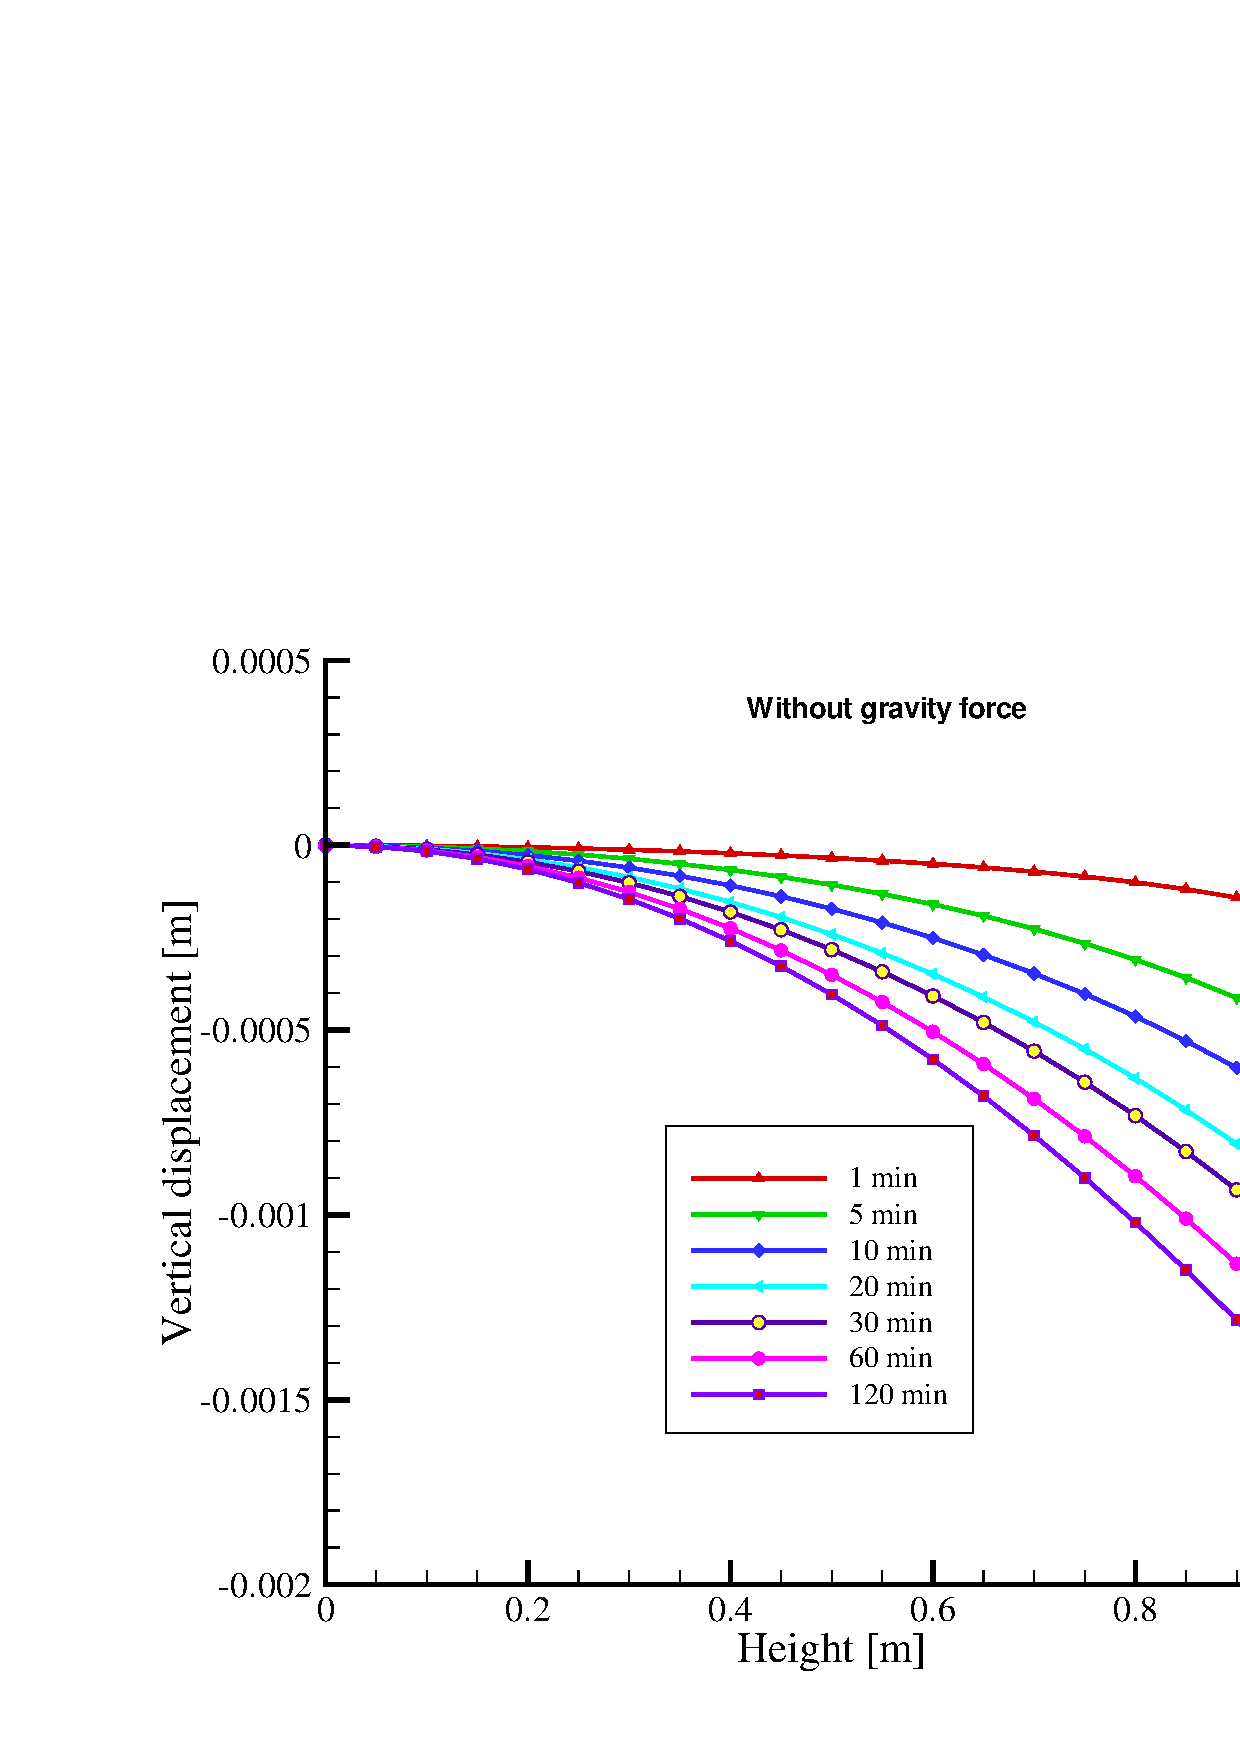
\includegraphics[width=0.49\textwidth]{chapter_14/figures/fig_14_2_13_c}
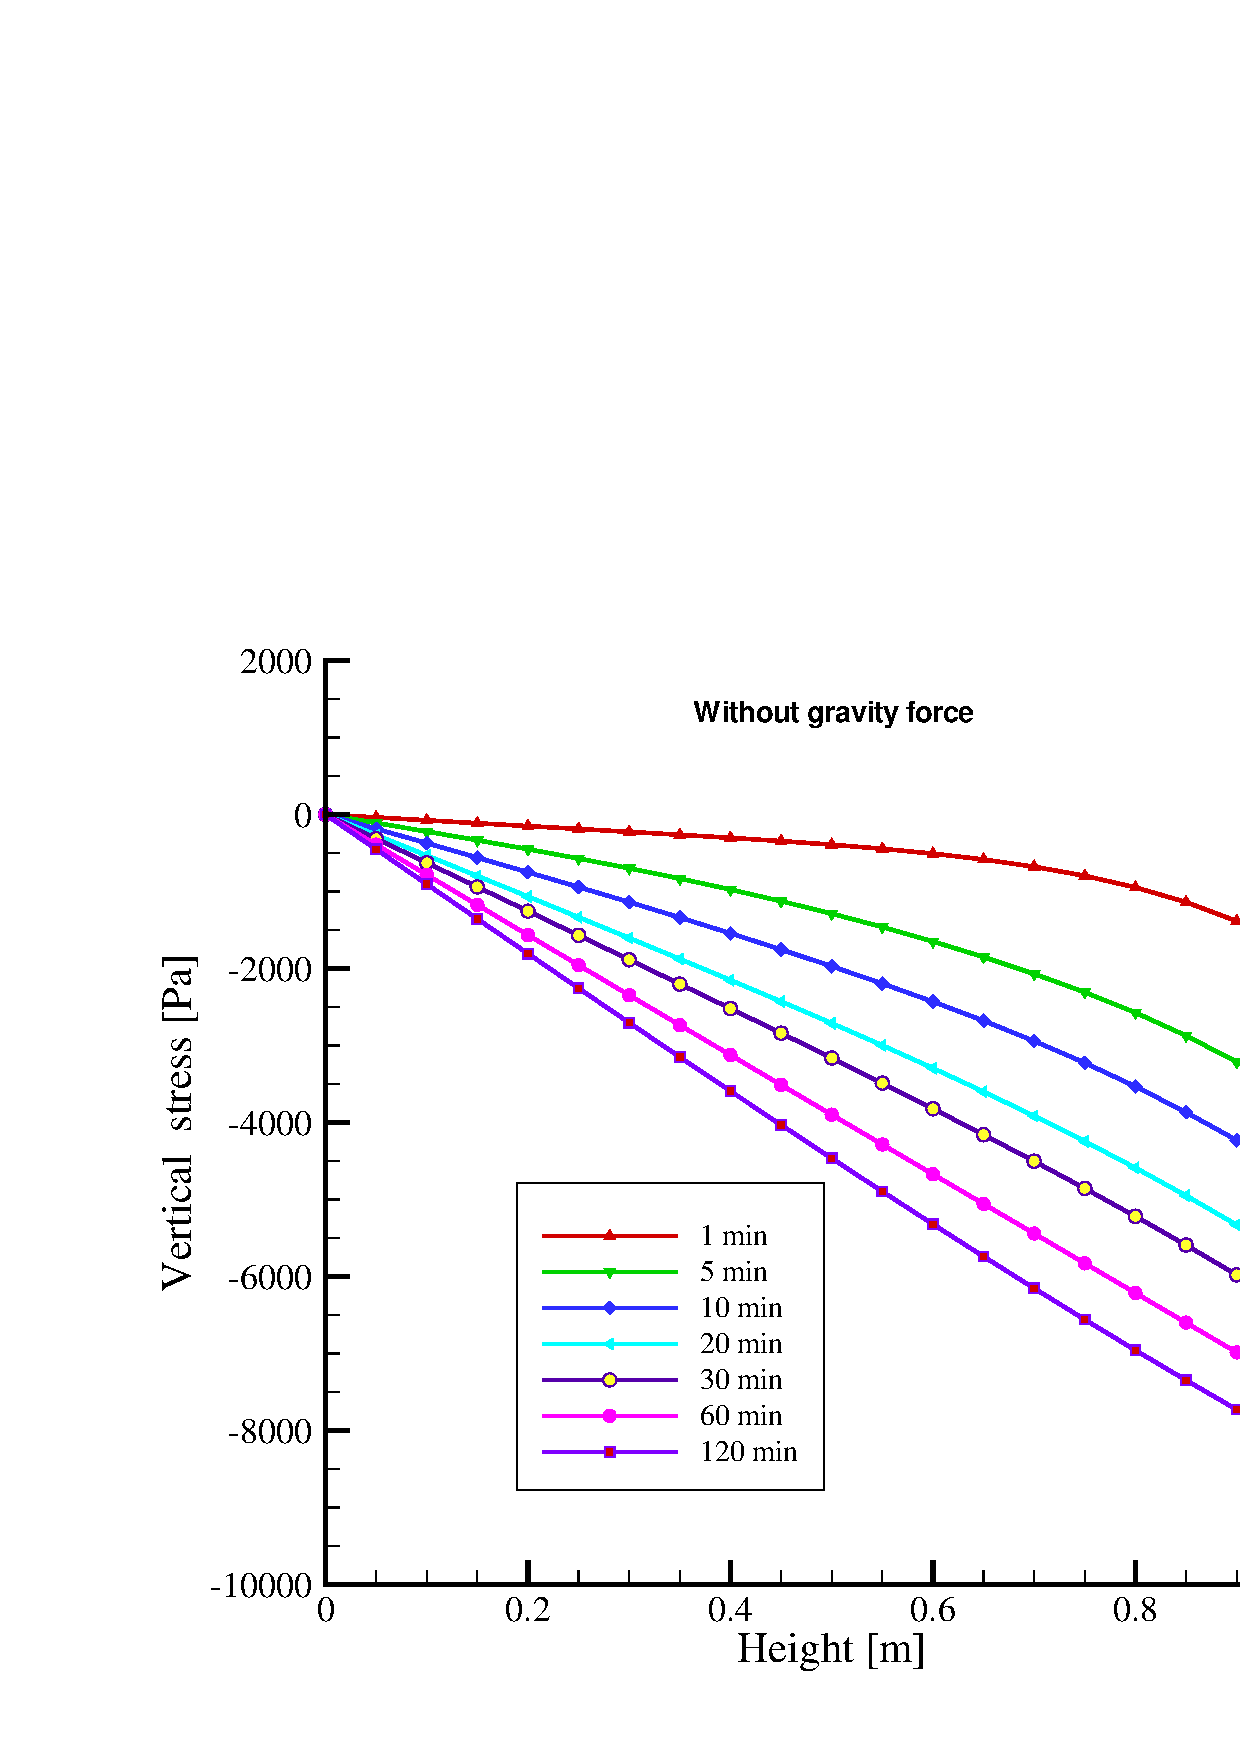
\includegraphics[width=0.49\textwidth]{chapter_14/figures/fig_14_2_13_d}
\end{center}
\caption{Simulated results without gravity force.}
\label{fig_HM_sat_nog}
\end{figure}

\begin{figure}[!t]
\begin{center}
\includegraphics[width=0.49\textwidth]{chapter_14/figures/fig_14_2_14_a}
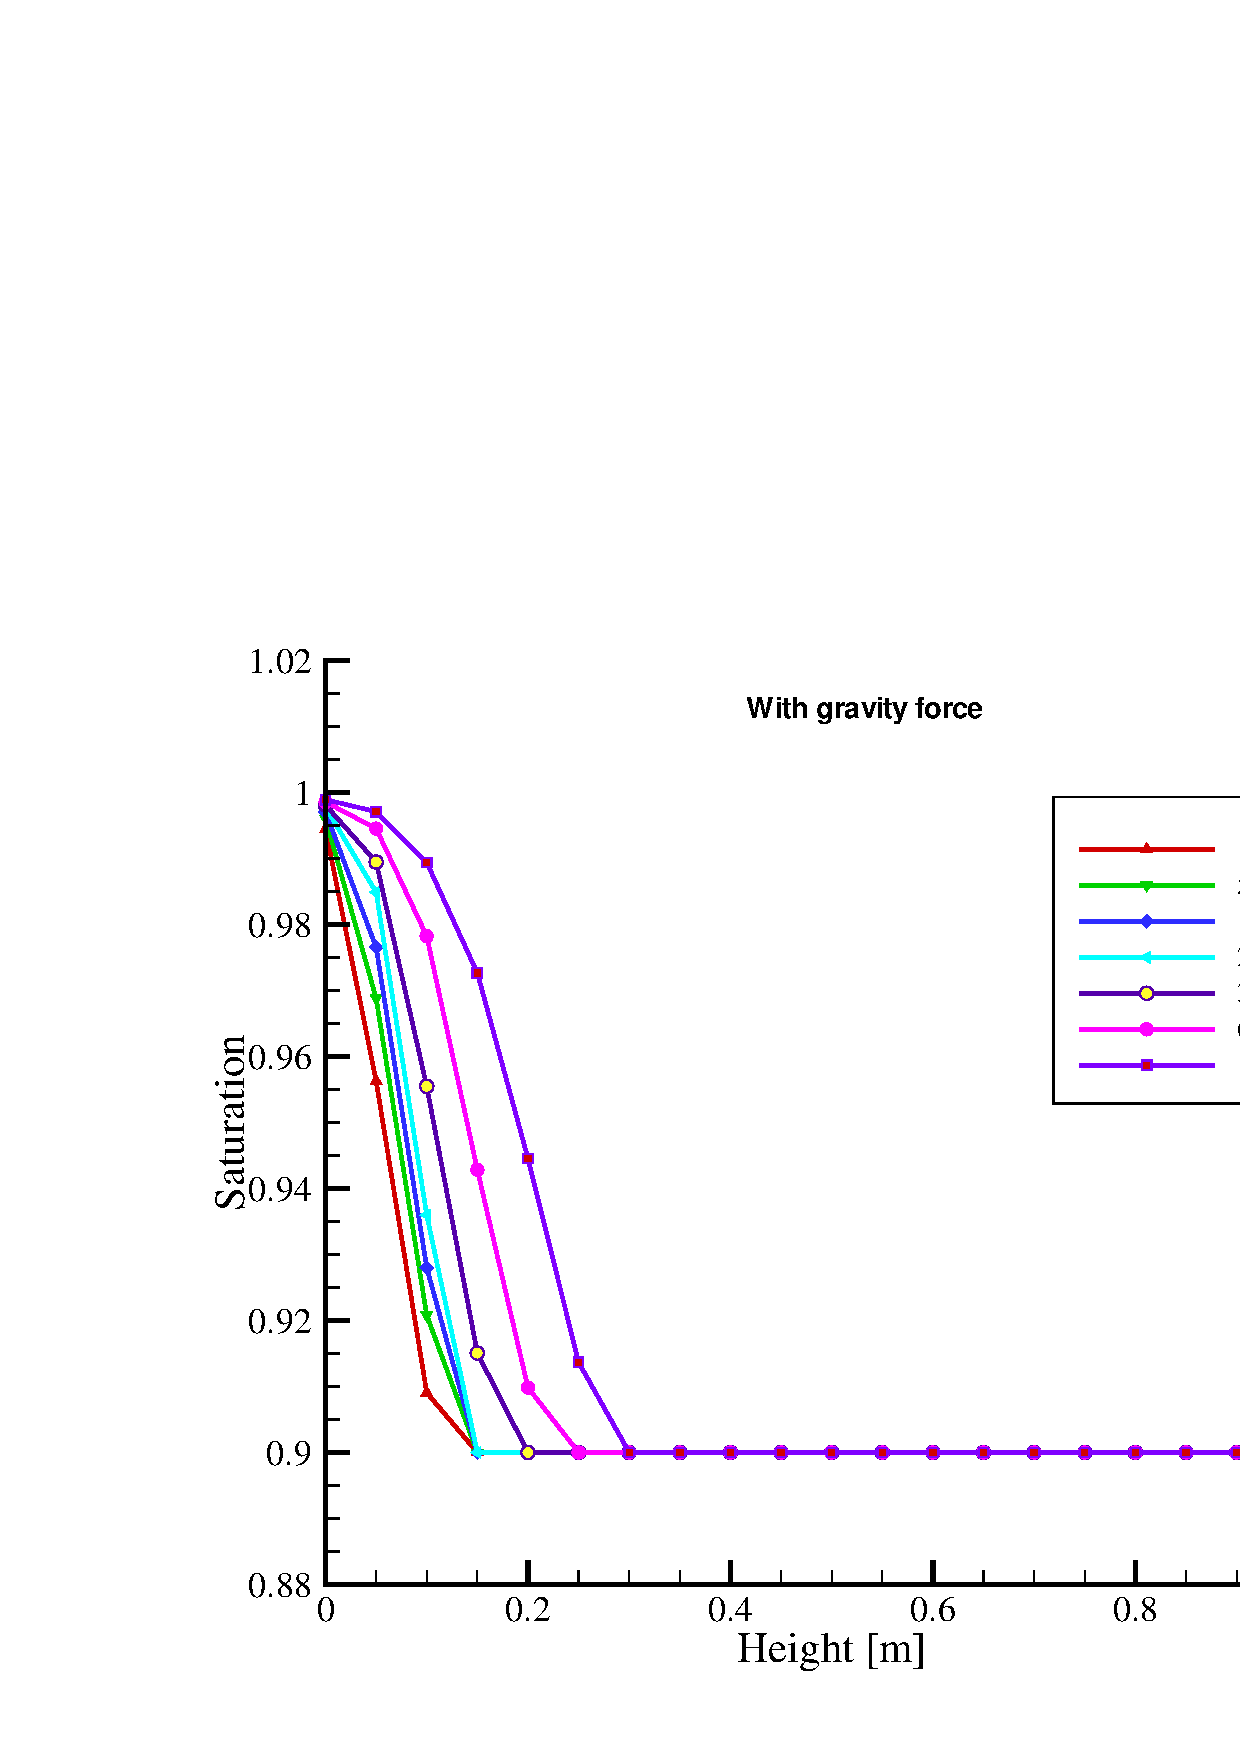
\includegraphics[width=0.49\textwidth]{chapter_14/figures/fig_14_2_14_b}
\includegraphics[width=0.49\textwidth]{chapter_14/figures/fig_14_2_14_c}
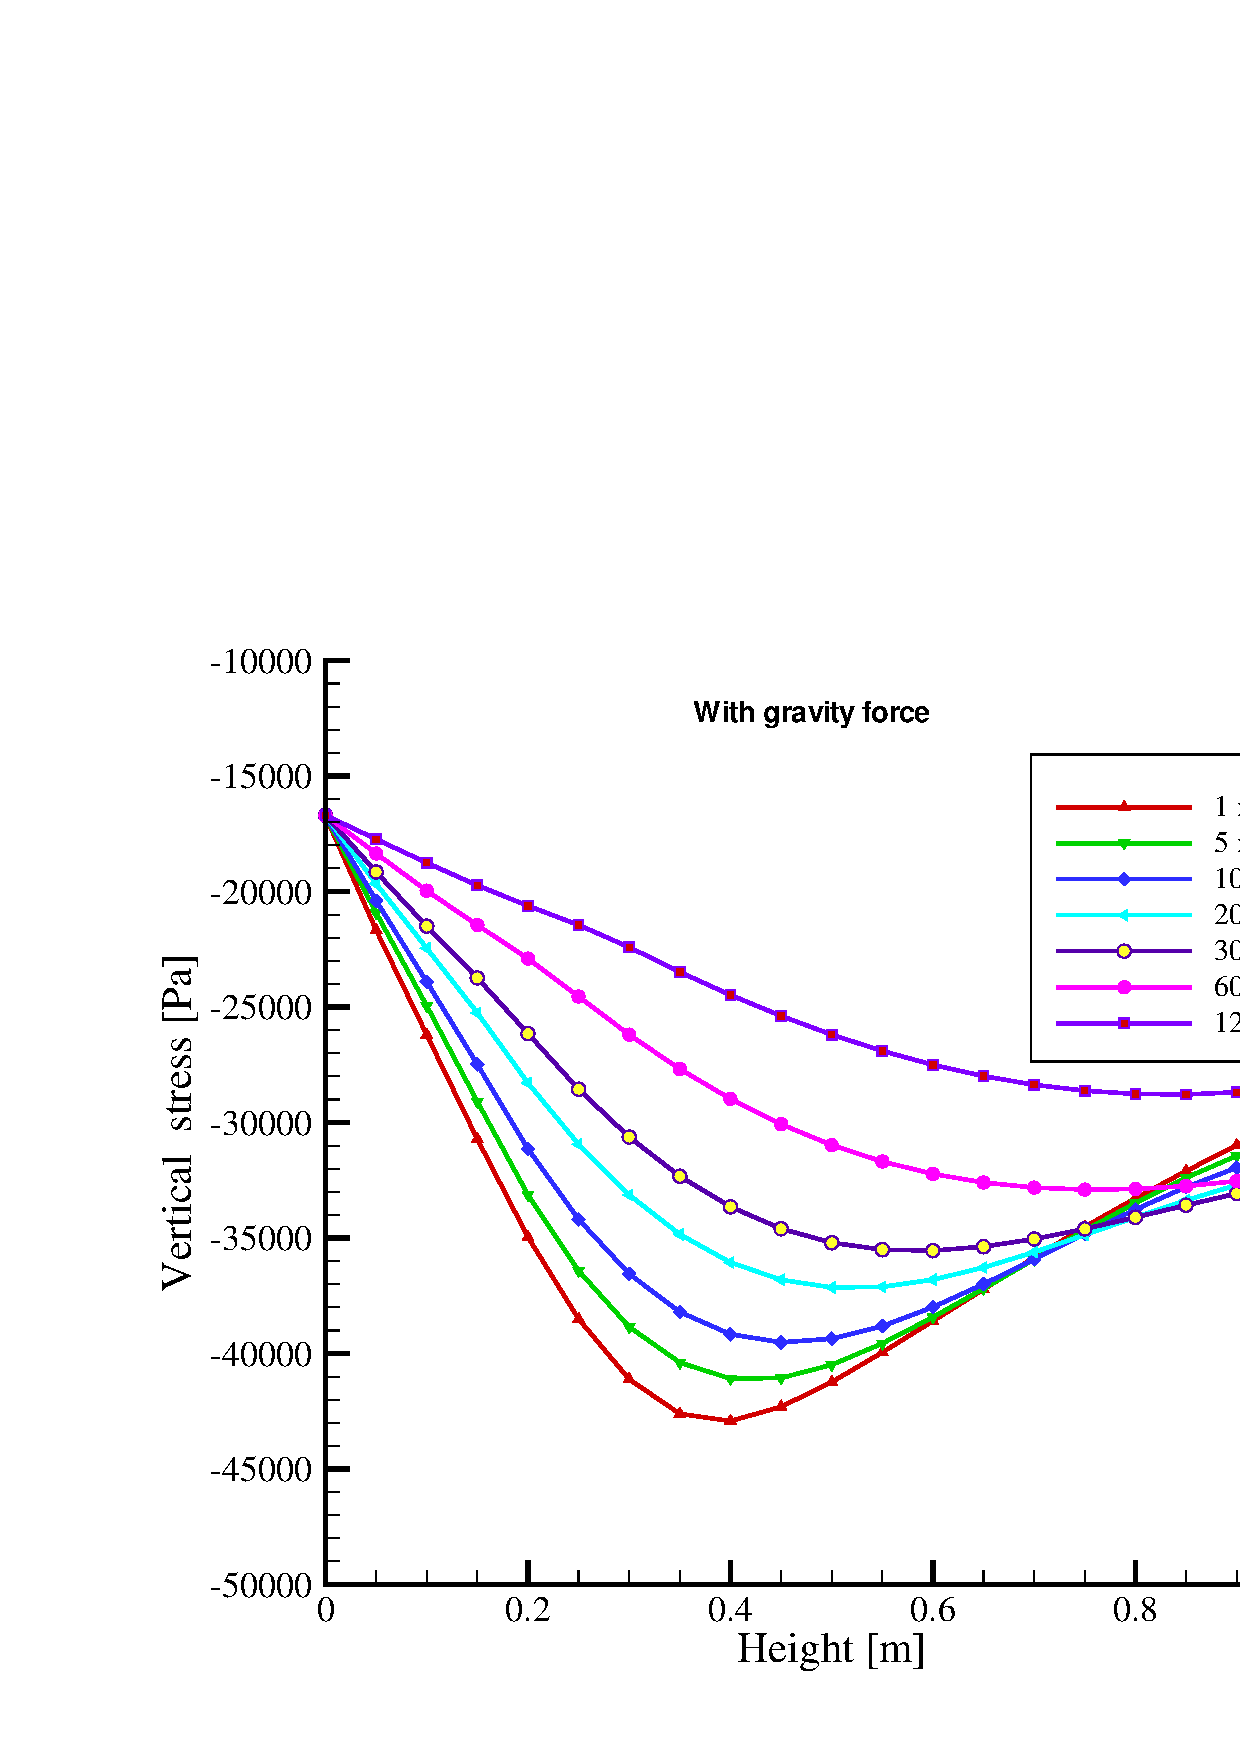
\includegraphics[width=0.49\textwidth]{chapter_14/figures/fig_14_2_14_d}
\end{center}
\caption{Simulated results with gravity force.}
\label{fig_HM_sat_g}
\end{figure}

\subsubsection*{Results}
We conduct two kinds of simulation: one including the gravity force as a load for the mechanical displacement field, and the other ignoring gravity. For the case of non-gravity, Fig. \ref{fig_HM_sat_nog} shows history profile of water pressure $p$, water saturation $S$, vertical solid displacement $u_y$ and vertical stress $\sigma _{yy}$.

The vertical profile of results obtained by taking into account the gravity force are shown in Fig. \ref{fig_HM_sat_g}. If compares the saturation result with that obtained by ignoring the gravity fore, one can easily see that the desaturation procedure is enhanced by the presence of solid gravity acting on the solid displacement field. This highlights the impact of displacement on water pressure and coupling effects between the two equation systems.
